\lstset{language=file,frame=single}

La Universidad Vecinal Ximena Yáñez Zapata
mantiene los datos de sus ramos en archivos de texto,
en los que cada línea corres\-ponde a un estudiante
y contiene varios datos separados por dos puntos («\verb+:+»)
como en el siguiente ejemplo:
\begin{verbatim}Martin:Soto:M:1990/8/24:39,86,22,56,30\end{verbatim}

Los datos de cada estudiante son, en orden:
el nombre, el ape\-llido,
el sexo (\verb+M+ si es masculino y \verb+F+ si es femenino),
la fecha de nacimiento (en formato \texttt{año/mes/día})
y las notas obtenidas (separadas por comas).

El archivo \texttt{progra.txt} contiene los datos
de los alumnos de la asignatura de Programística.

\newpage
\begin{certamen}[leftmargin=0pt]

  \item
    La dirección de email institucional
    está formada por
    la primera letra del nombre, un punto («\verb+.+»)
    y el apellido sin espacios,
    todo en minúsculas y seguido de \verb+@uvwyz.cl+.
    Escriba la función \verb!obtener_email(nombre, apellido)!:
\begin{lstlisting}[language=py,frame=none]
>>> obtener_email('Perico', 'Los Palotes')
'p.lospalotes@uvxyz.cl'
\end{lstlisting}

  \newpage
  \item
    A continuación,
    su equipo desarrollará un programa
    que gene\-rará una página web como la siguiente:

    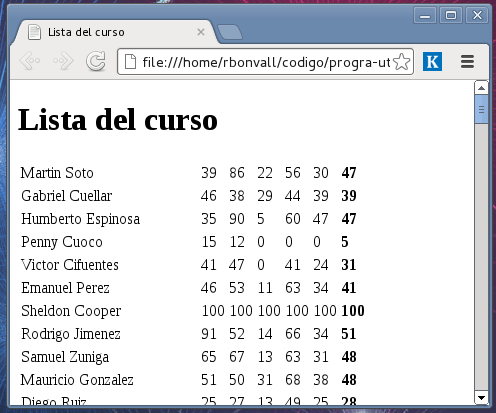
\includegraphics[width=0.8\textwidth]{curso-varias/pagina.png}

    La página web es simplemente un archivo de texto
    cuyo nombre tiene la extensión \texttt{.html}
    y cuyo contenido es algo como lo siguiente:

    \lstinputlisting[basicstyle=\small\ttfamily]{curso-varias/ejemplo.html}

    (Por brevedad aquí sólo se muestra los primeros dos estu\-diantes;
    usted debe agregarlos todos).
    Los datos listados son:
    el nombre completo,
    las notas de los cinco certámenes
    y el promedio final (encerrado entre \verb+<b>+ y \verb+</b>+).

    Su programa debe llamarse \texttt{pagina\_web.py},
    y debe generar un archivo llamado \texttt{progra.html}.
    Una vez creada,
    usted podrá abrir la página web con su navegador favorito.

  \newpage
  \item
    El profesor Rogelio Bombal de la asignatura de Programística
    desea enviar
    un email a cada estudiante para comunicarle su situación final
    al término del semestre.

    El contenido del email debe seguir el formato de este ejemplo:
    \lstinputlisting[language=]{curso-varias/Ignacio-Navarro.txt}

    Por supuesto,
    el email debe decir «aprobado» o «reprobado» según corresponda,
    y debe tratar a las damas de «estimada»
    y a los caballeros de «estimado».

    \newpage

    El archivo con el email debe llamarse
    \texttt{\textit{Nombre}-\textit{Apellido}.txt},
    reemplazando los espacios por guiones.
    Por ejemplo,
    el email para Rolando de la Cuadra
    debe estar en un archivo llamado \texttt{Rolando-de-la-Cuadra.txt}.

    La carita que va después de la nota
    depende del promedio obtenido:
    \framebox{\texttt{:'(}} si es menos de 35,
    \framebox{\texttt{:(}}  si está entre 35 y 54,
    \framebox{\texttt{:)}}  si está entre 55 y 84, y
    \framebox{\texttt{:D}}  si es 85 o más.

    Su equipo debe escribir el programa \verb!mails.py!.
    Este programa debe
    crear una carpeta llamada \verb!emails!,
    que contenga un archivo por cada alumno
    cuyo contenido sea el mensaje del profesor.

    Para crear la carpeta,
    use la función \li!makedirs!
    provista por el módulo \li!os!.
    Su único parámetro es el nombre de la carpeta.

    Para crear un archivo dentro de la carpeta \verb!emails!,
    debe indi\-car la carpeta y el nombre del archivo
    separados por una barra: \li!open('emails/archivo.txt', 'w')!.

%  \item
%
%    El profesor Rogelio Bombal desea publicar una página web
%    con los cumpleaños de los alumnos de Programística.
%
%    Escriba el programa \texttt{cumples.py},
%    que genere el archivo \texttt{cumples.html}.
%    El contenido de este archivo debe seguir la estructura
%    del ejemplo de más abajo.
%    (Por limitaciones de espacio,
%    aquí aparecen sólo los cumpleaños de los dos primeros meses.
%    Su programa debe incluírlos todos).
%
%    \begin{minipage}[T]{.40\textwidth}
%      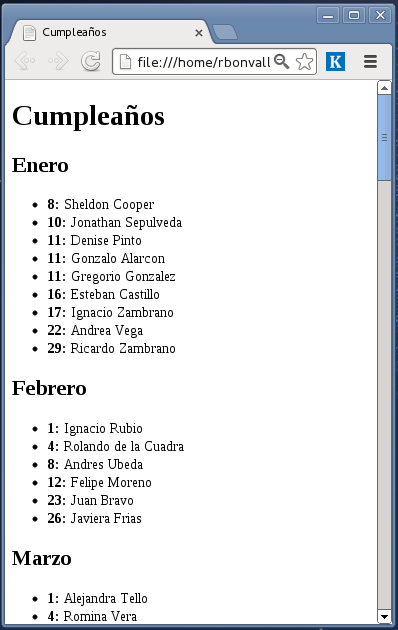
\includegraphics[width=\textwidth]{curso-varias/cumples.png}
%    \end{minipage}
%    \hfill
%    \begin{minipage}[T]{.55\textwidth}
%      Archivo \texttt{cumples.html}:
%      \lstinputlisting[basicstyle=\small\ttfamily]{curso-varias/ejemplo.html}
%    \end{minipage}
%
%  \newpage
%
%  \emph{(Opcional, sin nota).}
%  Modifique su programa para que
%  las personas que tienen cumpleaños el mismo día
%  sean mostrados en la misma línea:
%
%  \lstinputlisting[basicstyle=\small\ttfamily]{curso-varias/ejemplo-opcional.html}
%
%  Los nombres deben aparecer separados por comas,
%  excepto antes del último,
%  que debe estar precedido por «y».
%
%  \emph{(Opcional, sin nota).}
%  Modifique su programa para que el nombre de cada persona
%  sea un enlace para enviarle un mail.
%  Para esto, el nombre debe ser escrito en el archivo
%  como en el siguiente ejemplo:
%  \begin{lstlisting}
%<a href="mailto:a.vega@uvxyz.cl">Andrea Vega</a>
%  \end{lstlisting}

\end{certamen}
